\documentclass{article}
\usepackage{tikz}
\usepackage{comment}
\usetikzlibrary{positioning, arrows.meta, shapes.multipart, fit, calc}

\usepackage[a2paper, landscape, margin=2in]{geometry}

\begin{comment}
  Oxygen Not Included Seed Browser Frontend
  Copyright (C) 2025 The Maps Not Included Authors
  
  This program is free software: you can redistribute it and/or modify
  it under the terms of the GNU Affero General Public License as published by
  the Free Software Foundation, either version 3 of the License, or
  (at your option) any later version.
  
  This program is distributed in the hope that it will be useful,
  but WITHOUT ANY WARRANTY; without even the implied warranty of
  MERCHANTABILITY or FITNESS FOR A PARTICULAR PURPOSE.  See the
  GNU Affero General Public License for more details.
  
  You should have received a copy of the GNU Affero General Public License
  along with this program.  If not, see <http://www.gnu.org/licenses/>.
  
  See the AUTHORS file in the project root for a full list of contributors.
\end{comment}

\begin{comment}
  To compile this document to a PDF, use an appropriate LaTeX compiler.
  Tested to compile in Overleaf and in TeXeR.
\end{comment}

\begin{document}

\title{The Maps Not Included Atlas Feature Structure}

\date{June 2025}

\maketitle

Shared libraries:

\begin{itemize}
    \item mapsnotincluded.org/frontend/src/components/LoadImage.ts
    \item mapsnotincluded.org/frontend/src/components/MapData.ts
    \item mapsnotincluded.org/frontend/src/components/MediaToBase64.ts
    \item mapsnotincluded.org/frontend/src/components/CreateCascadingError.ts
\end{itemize}

\begin{center}
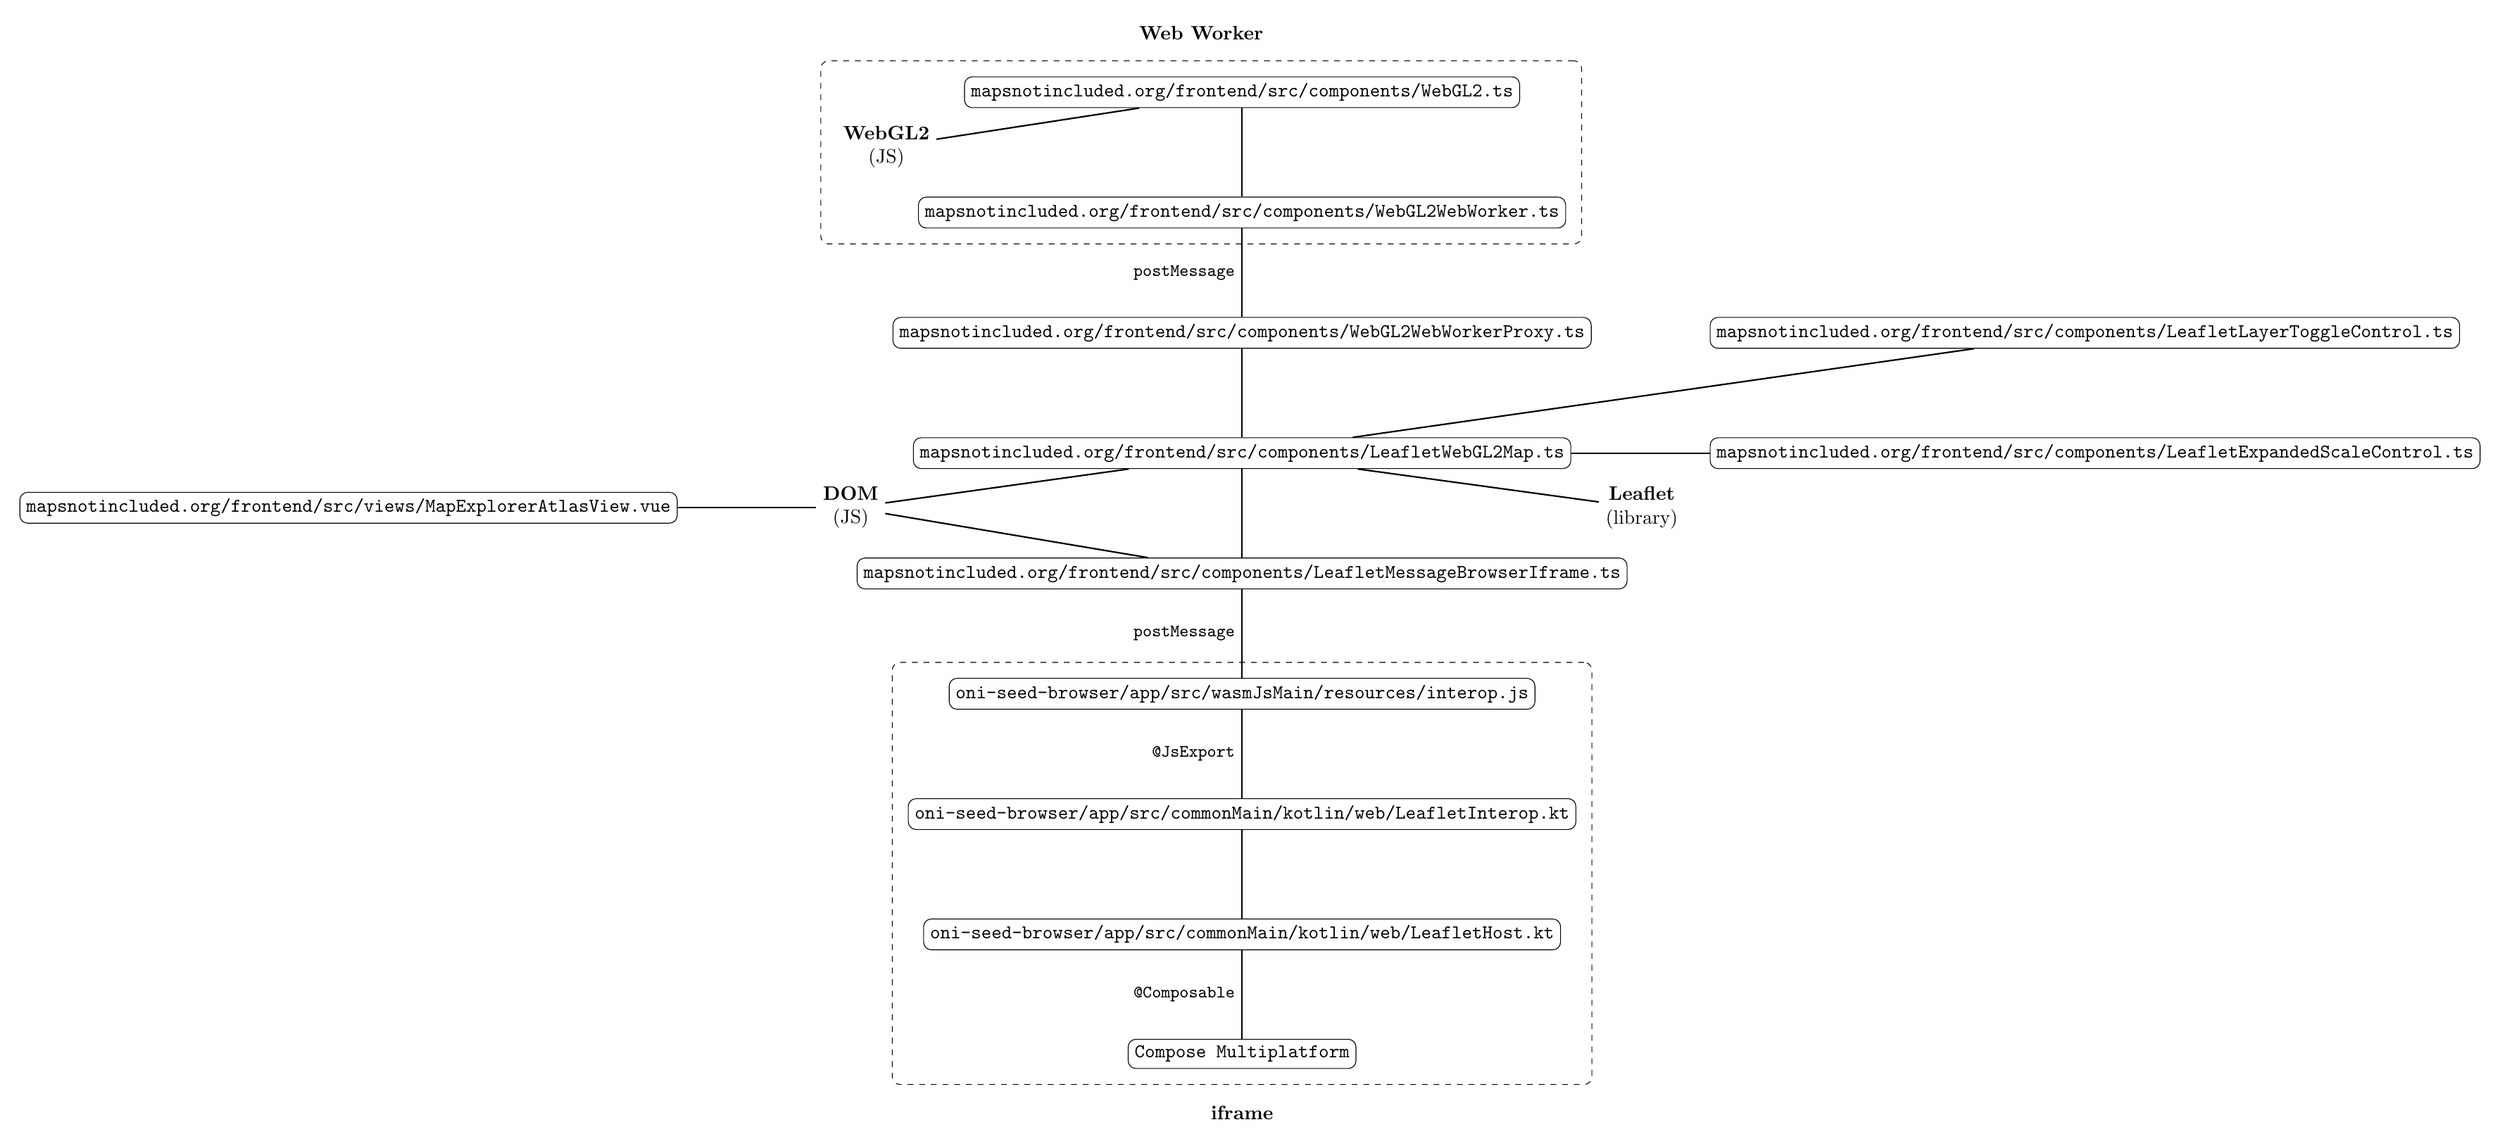
\begin{tikzpicture}[
    node distance=1.6cm and 2.5cm,align=center,
    module/.style={rectangle, draw, rounded corners, minimum height=1em, text centered, font=\ttfamily, fill=white},
    box/.style={draw, dashed, inner sep=8pt, rounded corners},
    arrow/.style={-, thick, >=Stealth},
    label/.style={font=\small\ttfamily}
]

% Main modules
\node[module] (webgl2) {mapsnotincluded.org/frontend/src/components/WebGL2.ts};
\node[module, below=of webgl2] (webglWorker) {mapsnotincluded.org/frontend/src/components/WebGL2WebWorker.ts};
\node[module, below=of webglWorker] (webglProxy) {mapsnotincluded.org/frontend/src/components/WebGL2WebWorkerProxy.ts};
\node[module, below=of webglProxy] (leafletMap) {mapsnotincluded.org/frontend/src/components/LeafletWebGL2Map.ts};
\node [module, right=of leafletMap] (expandedScale) {mapsnotincluded.org/frontend/src/components/LeafletExpandedScaleControl.ts};
\node [module, above right=of leafletMap] (toggleControl) {mapsnotincluded.org/frontend/src/components/LeafletLayerToggleControl.ts};
\node[module, below=of leafletMap] (iframeBridge) {mapsnotincluded.org/frontend/src/components/LeafletMessageBrowserIframe.ts};
\node[module, below=of iframeBridge] (interop) {oni-seed-browser/app/src/wasmJsMain/resources/interop.js};
\node[module, below=of interop] (kotlinInterop) {oni-seed-browser/app/src/commonMain/kotlin/web/LeafletInterop.kt};
\node[module, below=of kotlinInterop] (leafletHost) {oni-seed-browser/app/src/commonMain/kotlin/web/LeafletHost.kt};
\node[module, below=of leafletHost] (compose) {Compose Multiplatform};

% DOM and Leaflet labels
\node[below right=0.2cm and 0.5cm of leafletMap, align=center] (leafletLib) {\textbf{Leaflet}\\(library)};
\node[below left=0.2cm and 0.5cm of leafletMap, align=center] (dom) {\textbf{DOM}\\(JS)};
\node[below left=0.2cm and 0.5cm of webgl2, align=center] (webgl2Lib) {\textbf{WebGL2}\\(JS)};

\node[module, left=of dom] (view) {mapsnotincluded.org/frontend/src/views/MapExplorerAtlasView.vue};

% Boxes
\node[box, fit=(webgl2)(webglWorker)(webgl2Lib)] (workerbox) {};
\node at ($(workerbox.north) + (0,0.5)$) {\textbf{Web Worker}};
\node[box, fit=(compose)(interop)(kotlinInterop)(leafletHost)] (iframebox) {};
\node at ($(iframebox.south) - (0,0.5)$) {\textbf{iframe}};

% Arrows
\draw[arrow] (webgl2) -- (webgl2Lib);
\draw[arrow] (webgl2) -- (webglWorker);
\draw[arrow] (webglWorker) -- (webglProxy) node[midway, left, label] {postMessage};
\draw[arrow] (webglProxy) -- (leafletMap);
\draw[arrow] (iframeBridge) -- (interop) node[midway, left, label] {postMessage};
\draw[arrow] (interop) -- (kotlinInterop) node[midway, left, label] {@JsExport};
\draw[arrow] (kotlinInterop) -- (leafletHost);
\draw[arrow] (leafletHost) -- (compose) node[midway, left, label] {@Composable};
\draw[arrow] (iframeBridge) -- (leafletMap);
\draw[arrow] (iframeBridge) -- (dom);
\draw[arrow] (leafletMap) -- (expandedScale);
\draw[arrow] (leafletMap) -- (toggleControl);
\draw[arrow] (leafletMap) -- (dom);
\draw[arrow] (leafletMap) -- (leafletLib);
\draw[arrow] (dom) -- (view);

\end{tikzpicture}
\end{center}

\end{document}
